\documentclass[pdf, 9pt, usenames, dvipsnames, unicode, hyperref={bookmarks=true,bookmarksopen=false, bookmarksnumbered}]{beamer}
\setbeamersize{text margin left=0.8in,text margin right=0.8in}
\usepackage[T2A,T1]{fontenc}
\usepackage[english,russian]{babel}
\usepackage[utf8]{inputenc}
\usepackage{graphicx}
\usepackage{amsmath,amssymb,amsthm}
% \usepackage{anyfontsize}
\usepackage{tcolorbox}
\usepackage{amsfonts}
\usepackage{delarray}
\usepackage{multicol}
\usepackage{enumerate}
\usepackage{amsmath}
\usepackage{bm}
\graphicspath{{FIG/}}
\usefonttheme[onlymath]{serif}
\usepackage{beamerthemesplit}
\setbeamerfont{institute}{size=\normalsize}
\setbeamercolor{bluetext_color}{fg=blue}
\newcommand{\bluetext}[1]{{\usebeamercolor[fg]{bluetext_color}#1}}
\setbeamercovered{transparent}
\DeclareMathOperator{\sign}{sign}
\usepackage[update,prepend,suffix=]{epstopdf}
\newcommand{\alarm}[1]{\textcolor{red}{#1}}
\newcommand{\alarmg}[1]{\textcolor{blue}{#1}}
%%%%%%%%%%%%%%%%%%%%%%%%%%%%%%%%%%%%%%%%
% Изменение размеров footline
\defbeamertemplate*{footline}{my footline}{
  \leavevmode%
  \hbox{\begin{beamercolorbox}[wd=.2\paperwidth,ht=2.5ex,dp=1.125ex,leftskip=.3cm,rightskip=.3cm plus1fill]{author in head/foot}%
    \usebeamerfont{author in head/foot}\insertshortauthor
  \end{beamercolorbox}%
  \begin{beamercolorbox}[wd=.8\paperwidth,ht=2.5ex,dp=1.125ex,leftskip=.3cm,rightskip=.3cm plus1fil]{title in head/foot}%
    \usebeamerfont{title in head/foot}\insertshorttitle
  \end{beamercolorbox}}%
  \vskip0pt%
}\usebeamertemplate{my footline}
% Изменение размеров footline

% insert page numbers
\expandafter\def\expandafter\insertshorttitle\expandafter{%
  \insertshorttitle\hfill%
  \insertframenumber/\inserttotalframenumber}
% insert page numbers

%%%%%%%%%%%%%%%%%%%%%%%%%%%%%%%%%%%%%%%%
\setbeamercolor{bcgreen}{bg=green!100!black,fg=black}
\setbeamercolor{bcyellow}{bg=yellow!100!black,fg=black}
\setbeamercolor{bcred}{bg=red!100!black,fg=white}
\setbeamercolor{bcgray}{bg=white!80!black,fg=black}

\definecolor{anti-flashwhite}{rgb}{0.95, 0.95, 0.96}
\definecolor{blond}{rgb}{0.98, 0.94, 0.75}
\definecolor{brickred}{rgb}{0.8, 0.25, 0.33}

\title{Деревья решений}

\author[Гребенюк А.С.]
{Гребенюк А.С.}

\institute[shortinst]{Санкт-Петербургский государственный университет\\Прикладная математика и информатика\\ Кафедра Статистического Моделирования
}

\vspace{6mm}
\date{
	СПб, 2021\\[6mm]

}

\usepackage{cmap}

\begin{document}

%%%%%%%%%%%%%%%%%%%%%%%%%%%%%%%%%%%%%%%%%%%%%%%%%%%%
	
%%%%%%%%%%%%%%%%%%%%%%%%%%%%%%%%%%%%%%%%%%%%%%%%%%%%%%%%%%%%%%%%%%%%%%%%

\begin{frame}
\titlepage
\end{frame}

%%%%%%%%%%%%%%%%%%%%%%%%%%%%%%%%%%%%%%%%%%%%%%%%%%%%
	
\begin{frame}\frametitle{План доклада}

\begin{enumerate}
    \item Дерево
    \item Вероятностная постановка задачи
    \item Регрессионные деревья
    \item Классификационные деревья
        \begin{enumerate}
            \item Индекс Джини
            \item Кросс-энтропия
        \end{enumerate}
    \item Алгоритмы
        \begin{enumerate}
            \item CART
            \item ID3
            \item Стрижка деревьев
        \end{enumerate}
\end{enumerate}

\end{frame}
	
%%%%%%%%%%%%%%%%%%%%%%%%%%%%%%%%%%%%%%%%%%%%%%%%%%%%
	
\begin{frame}\frametitle{Дерево решений}

\begin{center}
    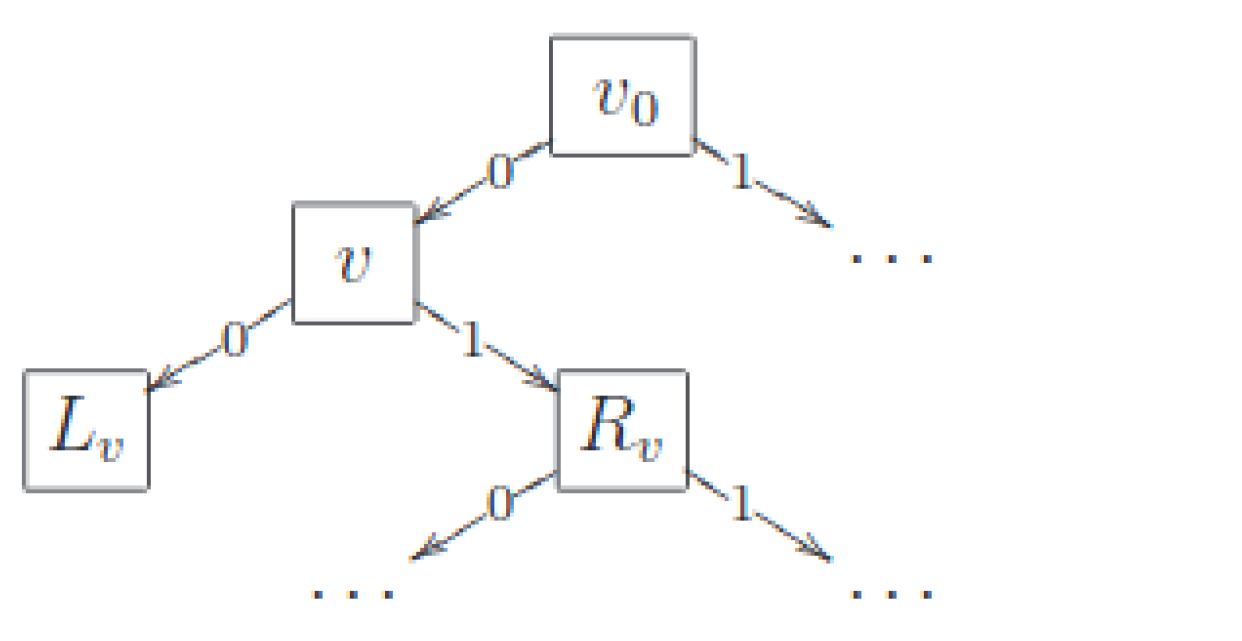
\includegraphics[scale=0.2]{pic2}
\end{center}

    \begin{center}
	Рис. . построение бинарного дерева решений
    \end{center}


\end{frame}

%%%%%%%%%%%%%%%%%%%%%%%%%%%%%%%%%%%%%%%%%%%%%%%%%%%%

\begin{frame}\frametitle{Дано}

Набор данных
$$\textbf{X} \in \mathbb{R}^{n \times p}.$$
Зависимые переменные
$$\textbf{y} \in \mathbb{R}^n.$$

$\textbf{x}_i \in \mathbb{R}^p$ --- вектор--строки $\textbf{X}$.\\
$X_j \in \mathbb{R}^n$ --- вектор--столбцы $\textbf{X}.$\\

$y \in \{1, \cdots, K \}$ --- задача классификации.\\
$y \in \mathbb{R}$ --- задача регрессии.\\

\end{frame}

%%%%%%%%%%%%%%%%%%%%%%%%%%%%%%%%%%%%%%%%%%%%%%%%%%%%

\begin{frame}\frametitle{Вероятностная постановка}

\begin{center}
    \textbf{Генеральная постановка}
\end{center}

Предполагаем, что $\eta$ и $\bm{\xi}$ функционально зависимы:

\begin{columns}

    \column{4.9 in}
    \begin{tcolorbox}[width=4.8in,left=0mm,right=0mm,top=0mm,bottom=0mm,boxrule=0pt]

    $$\eta = \varphi(\bm{\xi}) + \varepsilon,$$
    
\end{tcolorbox}
\end{columns}

$\varphi$ --- неизвестная функция.\\
$\eta \in \mathbb{R}$ --- случайная величина, зависимая переменная.\\
$\bm{\xi} \in \mathbb{R}^p$ --- случайный вектор, признаки.\\
$\varepsilon \in \mathbb{R}$ --- случайная величина, ошибка.\\

\begin{center}
    \textbf{Выборочная постановка}
\end{center}


\begin{columns}

    \column{4.9 in}
    \begin{tcolorbox}[width=4.8in,left=0mm,right=0mm,top=0mm,bottom=0mm,boxrule=0pt]

    $$y_i = \varphi(\textbf{x}_i) + \varepsilon_i,$$

\end{tcolorbox}
\end{columns}

\noindent$\varphi$ --- неизвестная функция.\\
$y_i$ --- реализация случайной величины $\eta$, зависимая переменная.\\
$\textbf{x}_i$ --- реализация случайного вектора $\bm{\xi}$, признаки.\\
$\varepsilon_i \in \mathbb{R}$ --- реализация случайной величины $\varepsilon$, ошибка.\\

\end{frame}

%%%%%%%%%%%%%%%%%%%%%%%%%%%%%%%%%%%%%%%%%%%%%%%%%%%%

\begin{frame}\frametitle{Регрессионные деревья}

\textbf{Выбор модели}
	$$\varphi(\textbf{x}_i, \bm{\Theta}) = \sum\limits_{j=1}^{J} c_j \mathbb{I}_{(\textbf{x}_i \in R_j)}.$$

\textbf{Выбор функции потерь}
	$$\text{RSS} = \sum\limits_{j=1}^{J} \sum\limits_{\textbf{x}_i \in R_j}^{} (y_i - \varphi(\textbf{x}_i, \bm{\Theta}))^2.$$

\textbf{Задача оптимизации}
	$$\text{RSS} = \sum\limits_{j=1}^{J} \sum\limits_{\textbf{x}_i \in R_j}^{} (y_i - \varphi(\textbf{x}_i, \bm{\Theta}))^2 \to \underset{R_1, \cdots, R_J}{\min}.$$
	
	$$\hat{c}_j = \dfrac{1}{|R_j|} \sum\limits_{\textbf{x}_i \in R_j} y_i.$$

\end{frame}

%%%%%%%%%%%%%%%%%%%%%%%%%%%%%%%%%%%%%%%%%%%%%%%%%%%%

\begin{frame}\frametitle{Пример регрессии}

    \begin{center}
    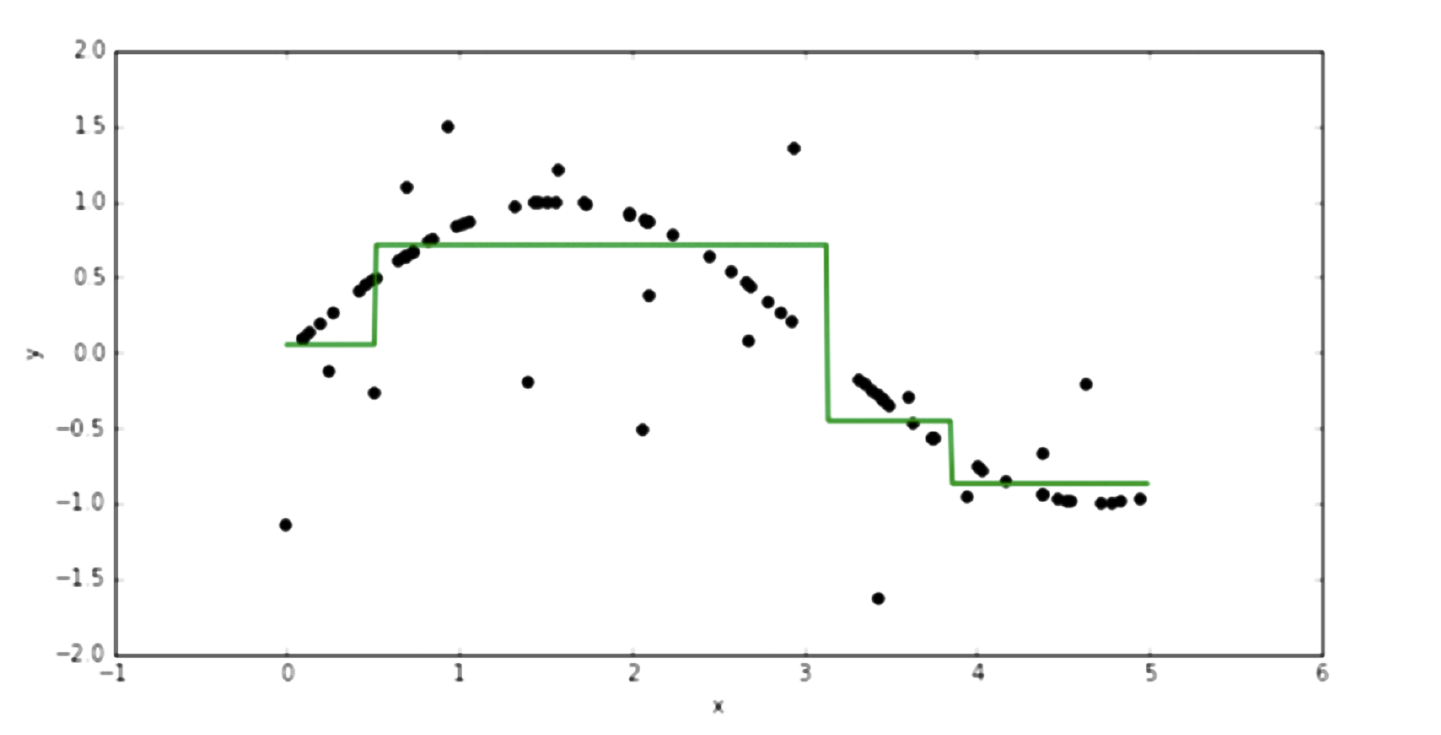
\includegraphics[scale=0.2]{pic31.png}{ \\ }
    \end{center}
    
    \begin{center}
	Рис. . регрессионная модель
    \end{center}
    
    \begin{center}
    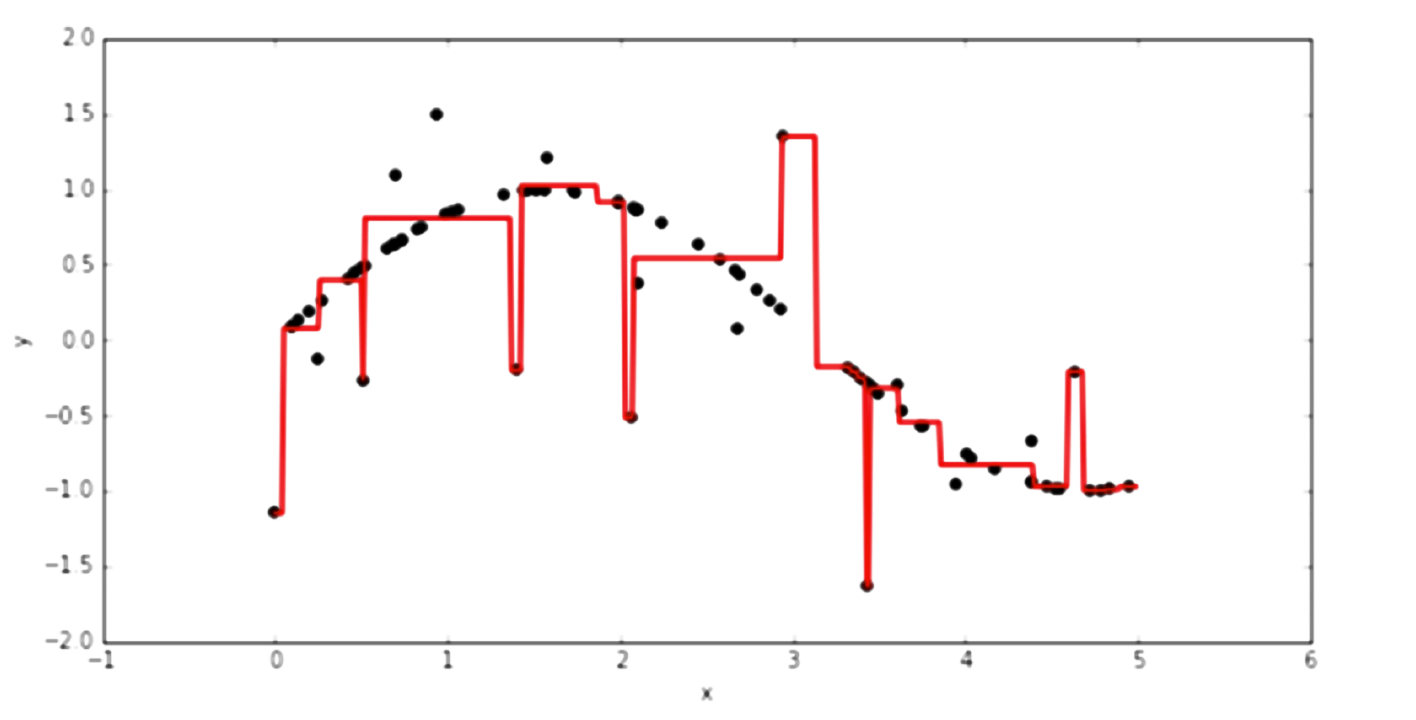
\includegraphics[scale=0.2]{pic32.png}{ \\ }
    \end{center}
    
    \begin{center}
	Рис. . переобученная регрессионная модель
    \end{center}


\end{frame}

%%%%%%%%%%%%%%%%%%%%%%%%%%%%%%%%%%%%%%%%%%%%%%%%%%%%

\begin{frame}\frametitle{Пример регрессии}

    \begin{center}
    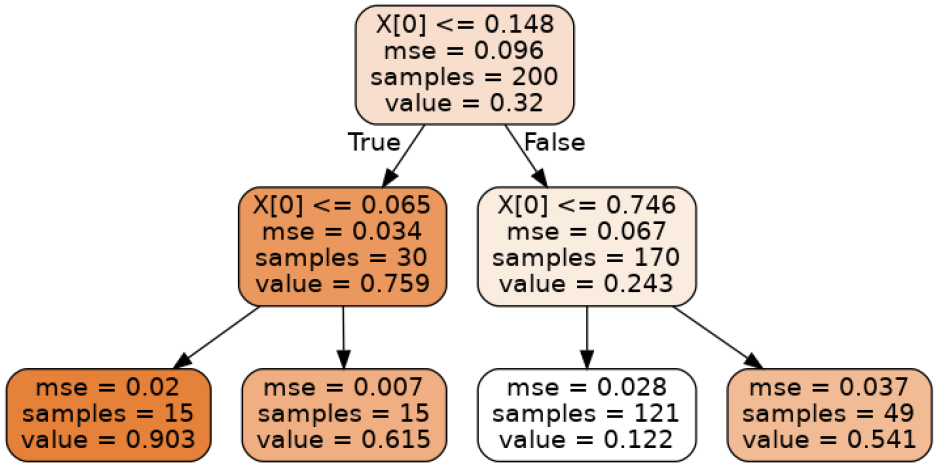
\includegraphics[scale=0.3]{pic101.png}{ \\ }
    \end{center}
    
    \begin{center}
	Рис. . регрессионное дерево решений
    \end{center}
    
    \begin{center}
    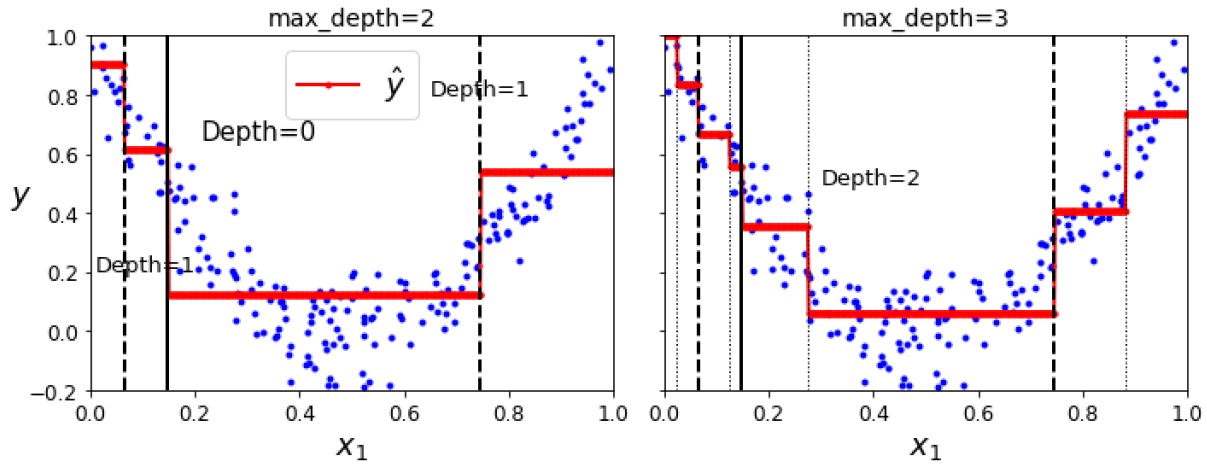
\includegraphics[scale=0.3]{pic102.png}{ \\ }
    \end{center}
    
    \begin{center}
	Рис. . модели регрессионного дерева решений
    \end{center}


\end{frame}

%%%%%%%%%%%%%%%%%%%%%%%%%%%%%%%%%%%%%%%%%%%%%%%%%%%%

\begin{frame}\frametitle{Классификационные деревья}

\textbf{Выбор модели}\\

	$$\varphi(\textbf{x}_i, \bm{\Theta}) = \sum\limits_{j=1}^{J} c_j \mathbb{I}_{(\textbf{x}_i \in R_j)}.$$

\textbf{Выбор функции потерь}\\

	$${p}_{jk} = \dfrac{1}{|R_j|} \sum\limits_{\textbf{x}_i \in R_j} Пусть \mathbb{I}_{(y_i = k)}$$ 
	${p}_{jk}$ --- доля объектов класса $k \in \{ 1, \cdots K \} $ в области $R_j$.\\

\end{frame}

%%%%%%%%%%%%%%%%%%%%%%%%%%%%%%%%%%%%%%%%%%%%%%%%%%%%

\begin{frame}\frametitle{Классификационные деревья}

\textit{Частота ошибок классификации}
$$E = \dfrac{1}{|R_j|} \sum\limits_{\textbf{x}_i \in R_j}^{} \mathbb{I}_{(y_i \neq k)}.$$

\textit{Индекс Джинни}
$$G = \sum\limits_{k=1}^{K} {p}_{jk}(1-{p}_{jk}),$$
$$G = 1 - \sum\limits_{k=1}^{K} p_{jk}^2.$$

\textit{Кросс-энтропия}
$$CI = - \sum\limits_{k=1}^{K} {p}_{jk} \log {p}_{jk}.$$

\end{frame}

%%%%%%%%%%%%%%%%%%%%%%%%%%%%%%%%%%%%%%%%%%%%%%%%%%%%

\begin{frame}\frametitle{Индекс Джини}

\begin{center}
	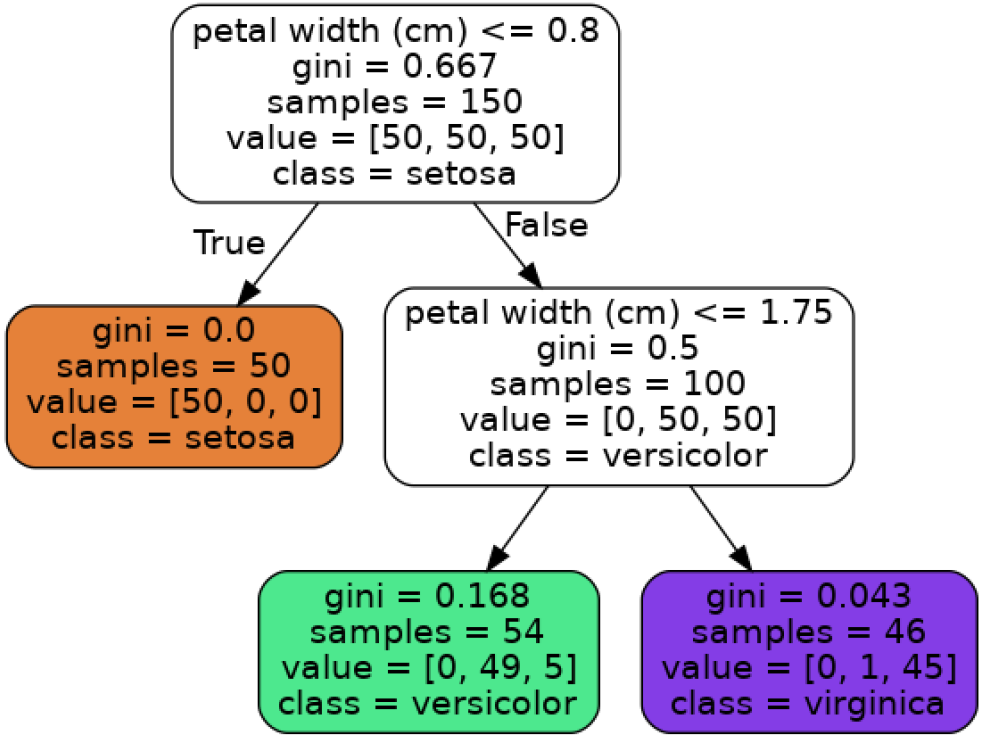
\includegraphics[scale=0.3]{piciris}
\end{center}
\begin{center}
	Рис. . дерево решений
\end{center}

\end{frame}

%%%%%%%%%%%%%%%%%%%%%%%%%%%%%%%%%%%%%%%%%%%%%%%%%%%%

\begin{frame}\frametitle{Индекс Джини}

Узел на глубине 0:
$$1 - \left(\dfrac{50}{150} \right)^2 - \left(\dfrac{50}{150} \right)^2 - \left(\dfrac{50}{150} \right)^2 = 1 - 3 \cdot \left(\dfrac{1}{3} \right)^2 = 1 - \dfrac{1}{3} = 0.666. $$ 

Узел на глубине 1 слева:
$$1 - \left( \dfrac{50}{50} \right)^2 - 0 - 0 = 0.$$

Узел на глубине 1 справа:
$$1 - 0 - \left( \dfrac{50}{100} \right)^2 - \left( \dfrac{50}{100} \right)^2 = 0.5. $$

Узел на глубине 2 слева:
$$1 - 0 - \left( \dfrac{49}{54} \right)^2 - \left( \dfrac{5}{54} \right)^2 = 0.168.$$

Узел на глубине 2 справа:
$$1 - 0 - \left( \dfrac{1}{46} \right)^2 - \left( \dfrac{45}{46} \right)^2 = 0.043.$$

\end{frame}

%%%%%%%%%%%%%%%%%%%%%%%%%%%%%%%%%%%%%%%%%%%%%%%%%%%%

\begin{frame}\frametitle{Impurity}

\begin{center}
	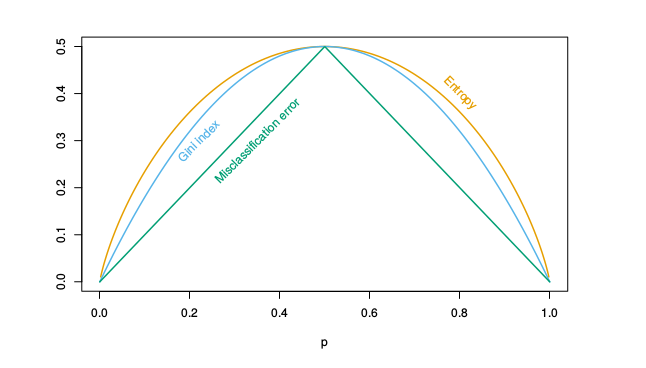
\includegraphics[scale=0.7]{pic5}
\end{center}
\begin{center}
	Рис. . Загрязненность \textit{impurity} узла для двухклассовой классификации измеряется как доля индивидов $p$, отнесенных ко второму классу
\end{center}

\end{frame}

%%%%%%%%%%%%%%%%%%%%%%%%%%%%%%%%%%%%%%%%%%%%%%%%%%%%

\begin{frame}\frametitle{Алгоритмы классификации}

\textbf{CART}

Разбиваем данные на две части
$$R_1(j,s) = \{ \textbf{x}_i \in \textbf{X} | X_j < s \}$$
и
$$R_2(j,s) = \{ \textbf{x}_i \in \textbf{X} | X_j \geq s \}.$$
\textbf{Оптимизационная задача}
$$\sum\limits_{i:\textbf{x}_i \in R_1 (j,s)} (y_i - \hat{c}_1) + \sum\limits_{i:\textbf{x}_i \in R_2 (j,s)} (y_i - \hat{c}_2) \to \min_{j,s}.$$

где где оценка коэффициента $\hat{c}_j = \dfrac{1}{|R_j|} \sum\limits_{\textbf{x}_i \in R_j(j,s)} y_i, \quad j = 1,2.$\\

Алгоритм CART --- жадный.

\end{frame}

%%%%%%%%%%%%%%%%%%%%%%%%%%%%%%%%%%%%%%%%%%%%%%%%%%%%

\begin{frame}\frametitle{Алгоритмы классификации}

\textbf{ID3}

\begin{enumerate}
	\item $\textbf{X}$ --- обучающая выборка, $\textbf{y} \in \{1, \cdots, k\}$.
	\item Если все $\textbf{x}_i$ имеют класс $k$, ставим метку 1 в корень и выходим из цикла.
	\item Если ни один $\textbf{x}_i$ не имеет класс $k$, ставим метку 0 в корень и выходим из цикла.
	\item Предикат $R(\textbf{x}_i):=\{ \textbf{x}_i | X_j \lessgtr s_j \}$ для которого информационная выгода наибольшая.
	\item Разбиваем $\textbf{X}$ на $\textbf{X}_0$ и $\textbf{X}_1$ по предикату $R$
	$$\textbf{X}_0:=\{ \textbf{x}_i \in \textbf{X}:R(\textbf{x}_i) = 0 \},$$
	$$\textbf{X}_1:=\{ \textbf{x}_i \in \textbf{X}:R(\textbf{x}_i) = 1 \}.$$
	\item Если $\textbf{X}_0 = \varnothing$ или $\textbf{X}_1 = \varnothing$, создаем новый лист $v$, $k_v$ --- класс, в котором находится большинство элементов $\textbf{x}_i.$
	\item Иначе создаем внутреннюю вершину $v$:
		\begin{enumerate}
			\item $R_v = R$;
			\item $L_v$;
			\item $R_v$.
		\end{enumerate}
\end{enumerate}

\end{frame}

%%%%%%%%%%%%%%%%%%%%%%%%%%%%%%%%%%%%%%%%%%%%%%%%%%%%

\begin{frame}\frametitle{Стрижка деревьев}

Описанный выше процесс может дать хорошие прогнозы на обучающем наборе, но, вероятно, \textit{переобучится}, что приведет к плохим результатам на тестовых наборах. Почему?

	$$\sum\limits_{j=1}^{|T|} \sum\limits_{\textbf{x}_i \in R_j}^{} (y_i - \hat{y}_{R_j})^2 + \alpha |T|.$$

\textbf{Критерий остановки}:\\
1. Ограничение макс. глубины дерева;\\
2. Ограничение мин. числа объектов в листе $n_{min}$;\\
3. Ограничение макс. количества листьев в дереве;\\
4. Остановка в случае, если все объекты в листе относятся к одному классу.

\end{frame}

%%%%%%%%%%%%%%%%%%%%%%%%%%%%%%%%%%%%%%%%%%%%%%%%%%%%

\begin{frame}\frametitle{Пример классификации: бейсбол}

Рассмотрим данные о зарплате в бейсболе. Заработная плата имеет цветовую маркировку от низкой (синий, зеленый) до высокой (желтый, красный).

\begin{center}
    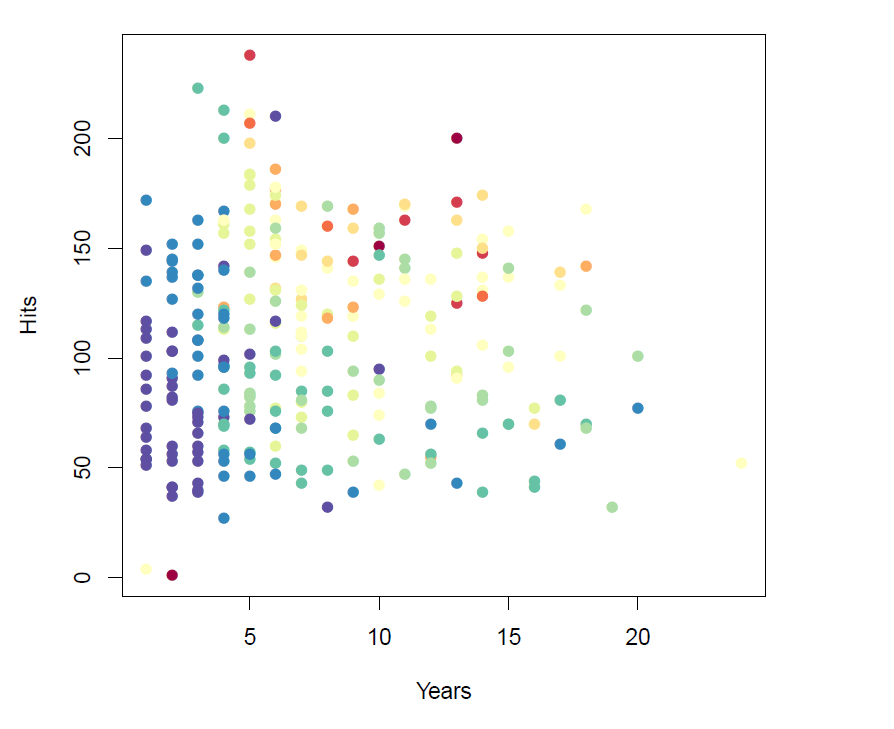
\includegraphics[scale=0.4]{pic61}
\end{center}

    \begin{center}
	Рис. . данные о бейсболе
    \end{center}


\end{frame}

%%%%%%%%%%%%%%%%%%%%%%%%%%%%%%%%%%%%%%%%%%%%%%%%%%%%

\begin{frame}\frametitle{Пример классификации: бейсбол}

	\begin{center}
	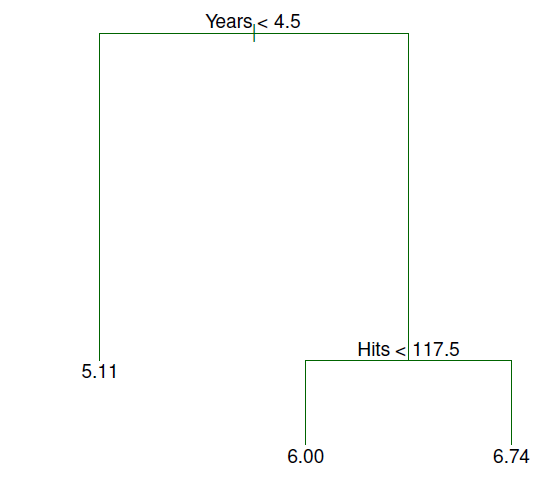
\includegraphics[scale=0.3]{pic62}
    \end{center}

	\begin{center}
	Рис. . классификационная модель
    \end{center}

    \begin{center}
	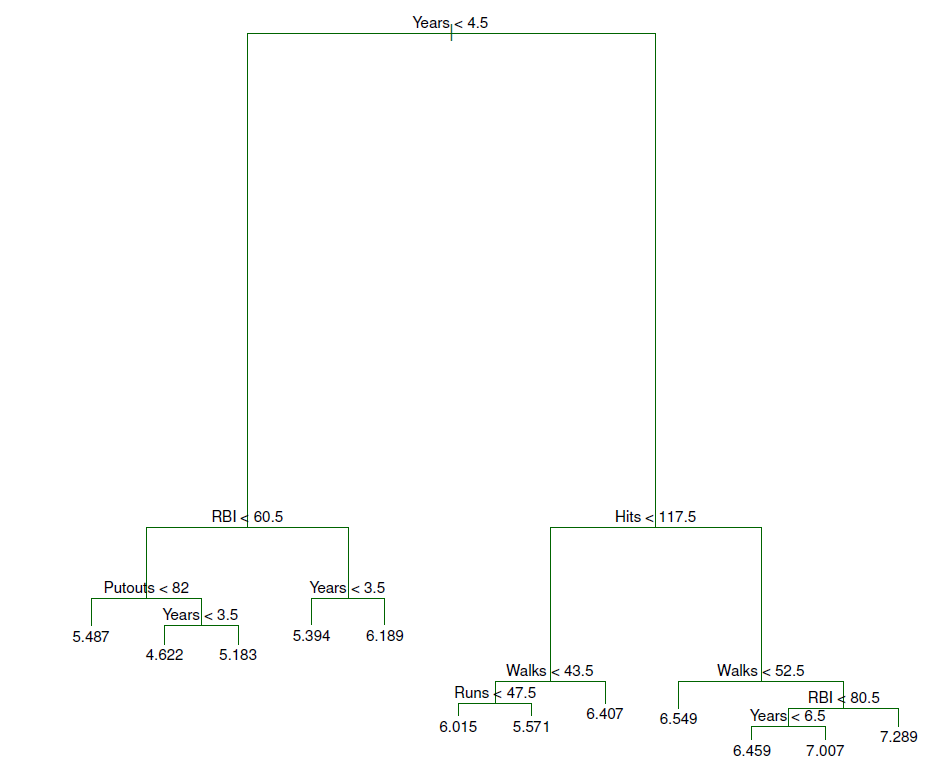
\includegraphics[scale=0.2]{pic63}
    \end{center}

    \begin{center}
	Рис. . переобученная классификационная модель
    \end{center}


\end{frame}

%%%%%%%%%%%%%%%%%%%%%%%%%%%%%%%%%%%%%%%%%%%%%%%%%%%%

\begin{frame}\frametitle{Пример классификации: бейсбол}

\begin{center}
	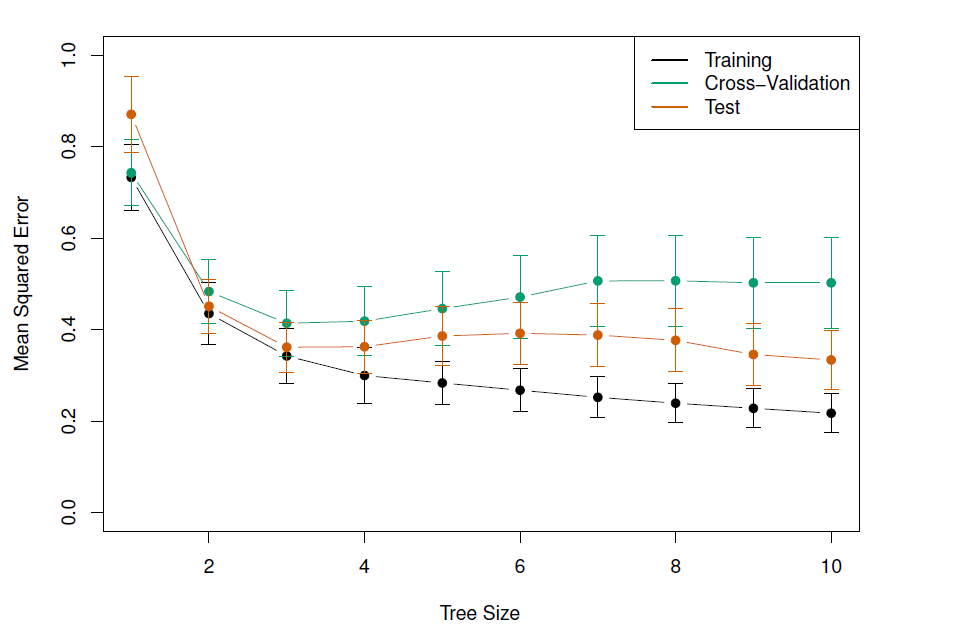
\includegraphics[scale=0.4]{pic64}
\end{center}

    \begin{center}
	Рис. . среднеквадратическая ошибка в зависимости от размера дерева
    \end{center}


\end{frame}

%%%%%%%%%%%%%%%%%%%%%%%%%%%%%%%%%%%%%%%%%%%%%%%%%%%%

\begin{frame}\frametitle{Пример классификации: бейсбол}

\begin{center}
	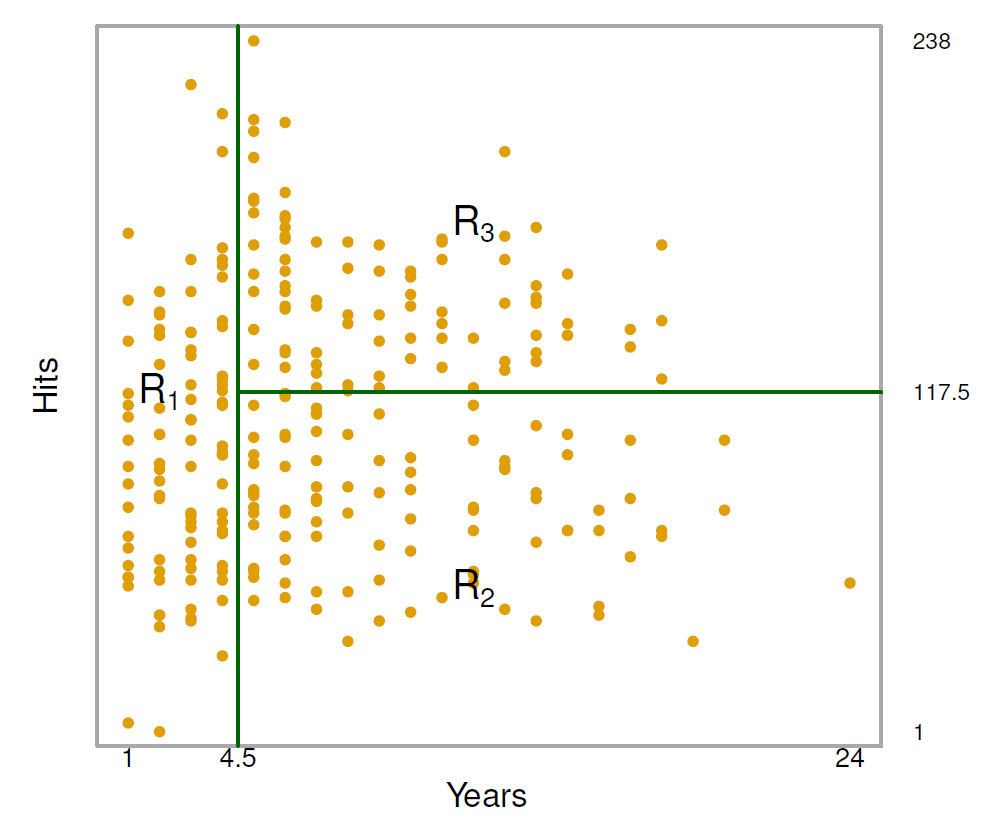
\includegraphics[scale=0.3]{pic65}
\end{center}

    \begin{center}
	Рис. . результат классификации
    \end{center}

$$R_1 = \{ X | Years < 4.5 \},$$
$$R_2 = \{ X | Years \geq 4.5, Hits < 117.5 \},$$
$$R_3 = \{ X | Years \geq 4.5, Hits \geq 117.5 \}.$$

\end{frame}

%%%%%%%%%%%%%%%%%%%%%%%%%%%%%%%%%%%%%%%%%%%%%%%%%%%%

\begin{frame}\frametitle{Пример классификации: сердце}

Эти данные содержат бинарный результат $HD$ для 303 пациентов с болью в груди.

\begin{center}
	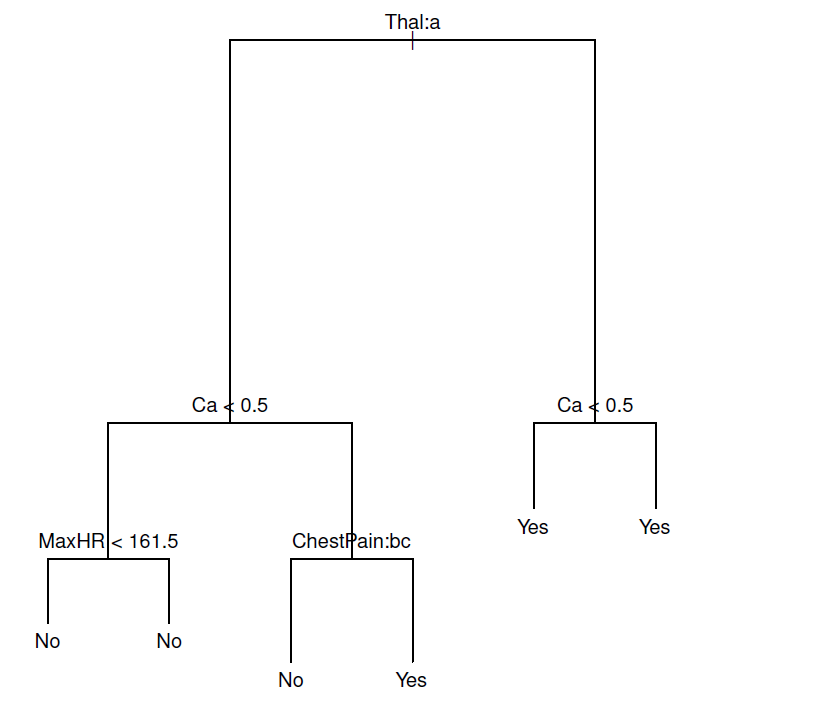
\includegraphics[scale=0.25]{pic71}
	
	\begin{center}
	Рис. . классификационная модель
    \end{center}

	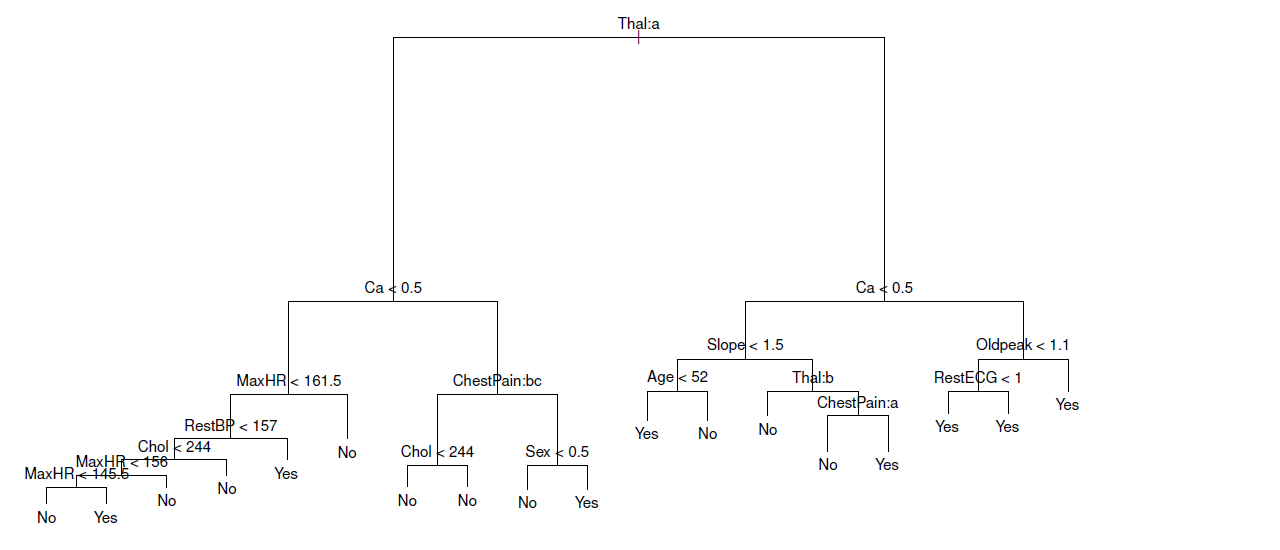
\includegraphics[scale=0.2]{pic72}
	
	\begin{center}
	Рис. . переобученная классификационная модель
    \end{center}

\end{center}

\end{frame}

%%%%%%%%%%%%%%%%%%%%%%%%%%%%%%%%%%%%%%%%%%%%%%%%%%%%

\begin{frame}\frametitle{Пример классификации: сердце}

\begin{center}
	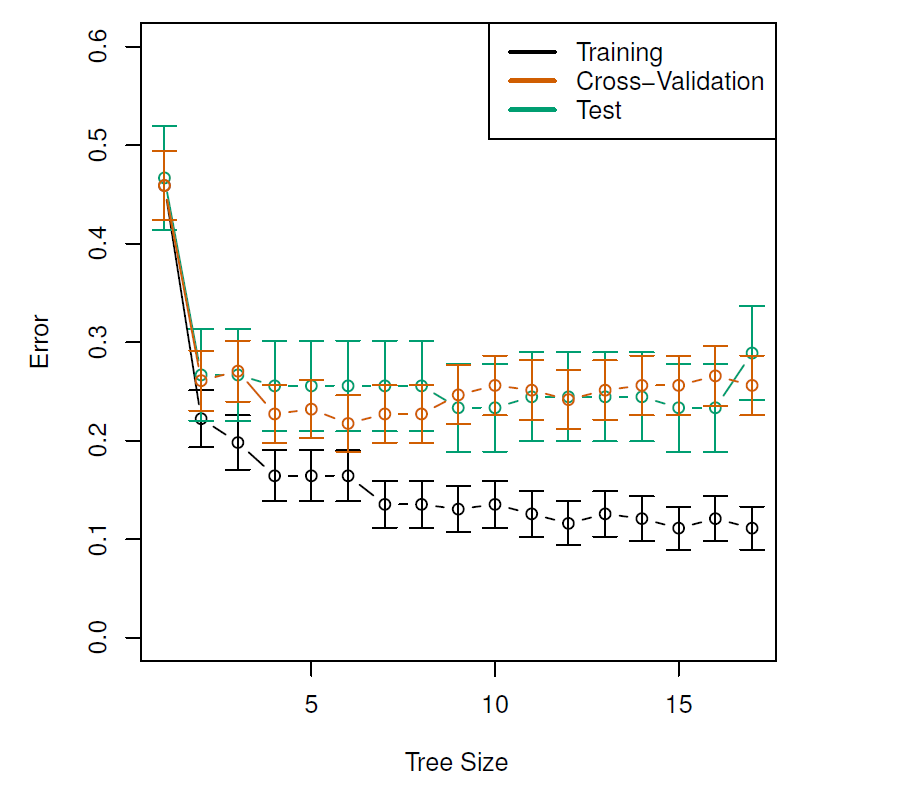
\includegraphics[scale=0.3]{pic73}
\end{center}

    \begin{center}
	Рис. . среднеквадратическая ошибка в зависимости от размера дерева
    \end{center}


\end{frame}

%%%%%%%%%%%%%%%%%%%%%%%%%%%%%%%%%%%%%%%%%%%%%%%%%%%%

\begin{frame}\frametitle{Сравнение деревьев с линейными моделями}

\begin{center}
	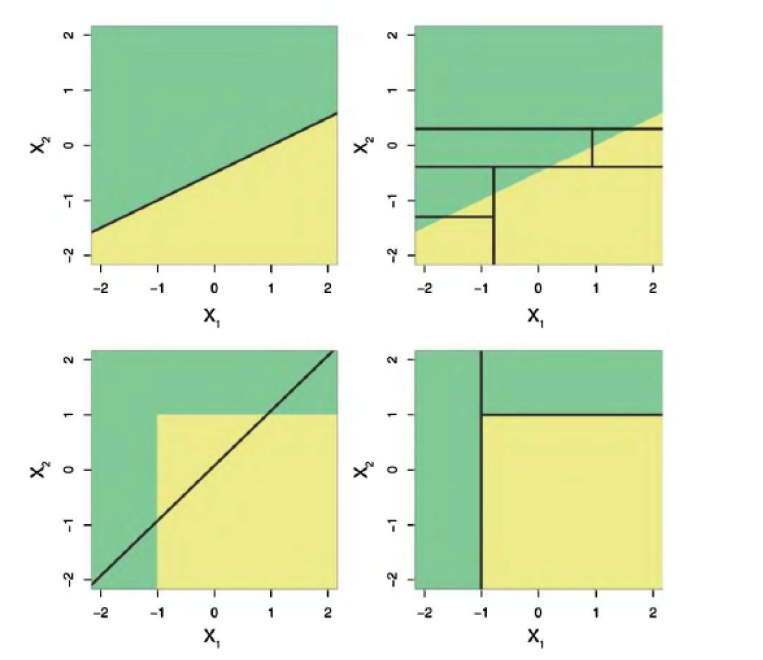
\includegraphics[scale=0.4]{pic10}
\end{center}
\begin{center}
	Рис. . сравнение моделей
\end{center}
\end{frame}

%%%%%%%%%%%%%%%%%%%%%%%%%%%%%%%%%%%%%%%%%%%%%%%%%%%%

\begin{frame}\frametitle{Преимущества и недостатки рещающих деревьев}

\textbf{Преимущества}:\\
1. Классификация + регрессия.\\
2. Легко визуализировать.\\
3. Легко интерпретировать.\\
4. Интуитивность.

\textbf{Недостатки}:\\
1. Небольшая точность.\\
2. Переобучение.

\end{frame}

% \begin{tcolorbox}[width=4.8in,left=0mm,right=0mm,top=0mm,bottom=0mm,boxrule=0pt]
% \begin{tcolorbox}[width=4.8in,left=0mm,right=0mm,top=0mm,bottom=0mm,colback=orange!50!white,boxrule=0pt] 
% \begin{tcolorbox}[width=4.8in,left=0mm,right=0mm,top=0mm,bottom=0mm,colback=Yellow!70!white,boxrule=0pt]

\end{document}